\chapter{Results} \label{results}
This chapter will encompass the result of the two ML models for NBRA prediction as well as the evaluation of the in-situ interviews and the passive observation statistic of NBRAs.
\subsection{Data-processing} \label{results_dataprocessing}
The following table \ref{tab:data_reduction_values}will provide data-reduction values for each data-source and data-set used. These reductions were the result of the different data-processing steps described in \ref{sec:} which will be shortly listed again below:
\begin{itemize}
  \item in boundary check
  \item dominant authors exclusion
  \item bulk uploads
\end{itemize}

\begin{table}[ht]
\begin{center}
\caption{Data-reduction according to the different data-sources as a result of data-processing steps}\vspace{1ex}
\label{tab:data_reduction_values}
\begin{tabular}{llccc}\hline
data-set & top authors excluded & bulk threshold & input & output & data-reduction\\ \hline
Instagram Zug & 6 & 6 & 28'246 & 11'777 & 58.3\% \\
Instagram Zurich Uetliberg & 10 & 5 & 74'742 & 68'522 & 8.3\% \\
Instagram Zurich Dolder & 7 & 5 &  206'454 &  191'584 & 7.2\% \\
Flickr Zug & 12 & 7 &  14'236 &  3'790 & 73.4\% \\ 
Foursquare Zug & - & - & 405 & 405 & 0.0\% \\ \hline
\end{tabular}
\end{center}
\end{table}

The noticeably high data-reduction of the Flickr data-set was mostly due to high user upload activity. As seen in \ref{img:dominant_users_flickr} a small portion of Flickr-users (authors) uploading up to  1'190 posts since the SMP Flickr was launched in 2005 account for a big share of the entire data-set. As a result to reduce this bias, roughly 5'700 media objects were removed alone in the 'dominant user' data-processing step.\\
Similar graphs to \ref{img:dominant_users_flickr} were created for all the data-sets according to which the thesis author decided the thresholds in \ref{tab:data_reduction_values} manually. 

\begin{figure}[ht]
   \centering
   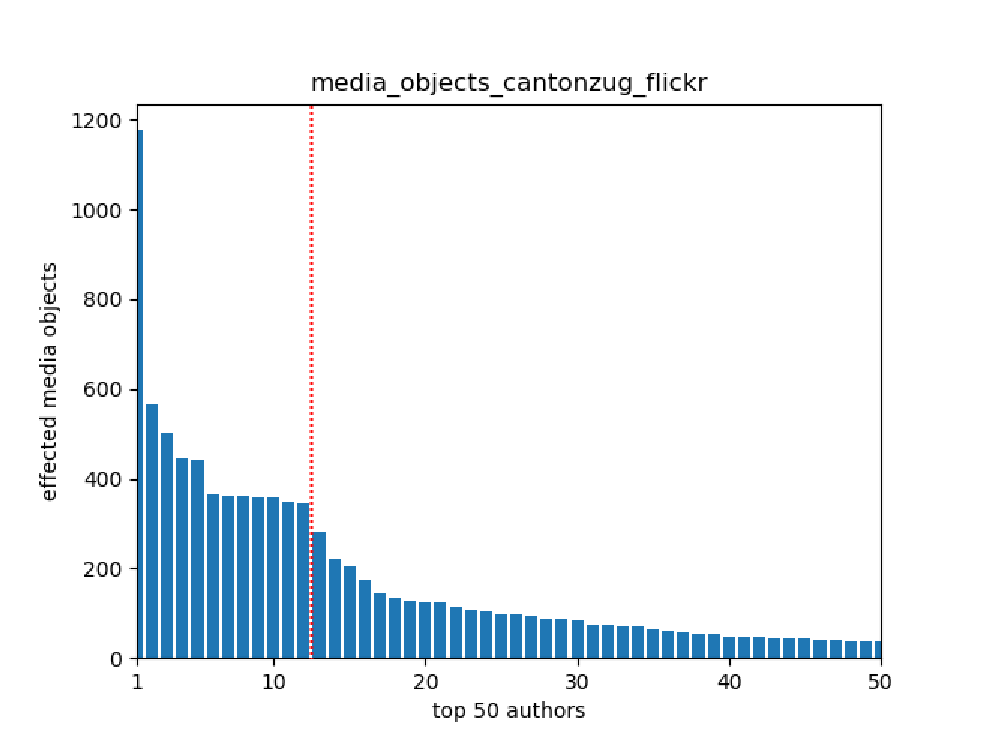
\includegraphics[width=0.75\textwidth]{img/cantonzug_flickr_top50_w_line}
   \caption{The top 12 Flickr authors which account for roughly 5'700 media objects (left to the red line) were excluded from further data-analysis}
   \label{img:dominant_users_flickr}
\end{figure}



\subsection{Model performance}

